 \chapter{Data Collection}
 Our main dataset is a connected corpus of news articles about the presidential elections and the tweets that share them from January 1, 2016 to May 1, 2016 over 13 news outlets. In this chapter, we detail the collection and creation of our dataset, along with the unique challenges of working with ``big data''.

\section{The Electome Project}
The backbone of our data collection and classification process lies under the umbrella of the Electome project, a large, collaborative effort with the Laboratory for Social Machines to examine the ``horse-race of ideas'' and competition of narratives during the presidential election year. The goal of the Electome project is to create novel stories for data journalists as well as technically innovative ways to examine the national conversation using machine learning and ``big data'' analysis through both social and traditional media coverage. The first step of both our news and Twitter data processing method uses machine learning classifiers from the Electome project.

\section{News Dataset}

 \subsection{Duration \& Scope}
 For our news dataset, we scraped articles from the RSS feeds of news publications every hour over five months and 13 publications:

\begin{multicols}{2}
\begin{itemize}

\item CNN
\item Fox News
\item The New York Times
\item The Wall Street Journal
\item The Washington Post
\item The Los Angeles Times 
\item The Associated Press
\item Reuters
\item McClatchy 
\item Politico 
\item Buzzfeed
\item The Huffington Post
\item NPR 
\end{itemize}
\end{multicols}

The choices above span a mix of publications. We include sources that: 

\begin{itemize}
\item Have mostly conservative audiences and mostly liberal audiences \cite{PoliticalPolarization}
\item Come from mixed primary media formats (television, paper, online, radio)
\item Are viewed as ``legacy'' (over a hundred years old) and ``new'' media (founded online within the last 10 years)
\item Focus solely on political news (Politico, McClatchy)
\item Are newswire services (the Associated Press, Reuters news)
\end{itemize}
 
 to capture a variety of types of election coverage and target audiences.
 
 We look at stories from January 1, 2016 (the start of the election year) to May 1, 2016. This time period captures the bulk of the primary election, when coverage of multiple presidential candidate contenders creates greater variety in news stories for our analysis.
  
\subsection{Data Pipeline}

Articles are processed in a 3-step pipeline, pictured below.

\begin{figure}[H]  
\centering 
  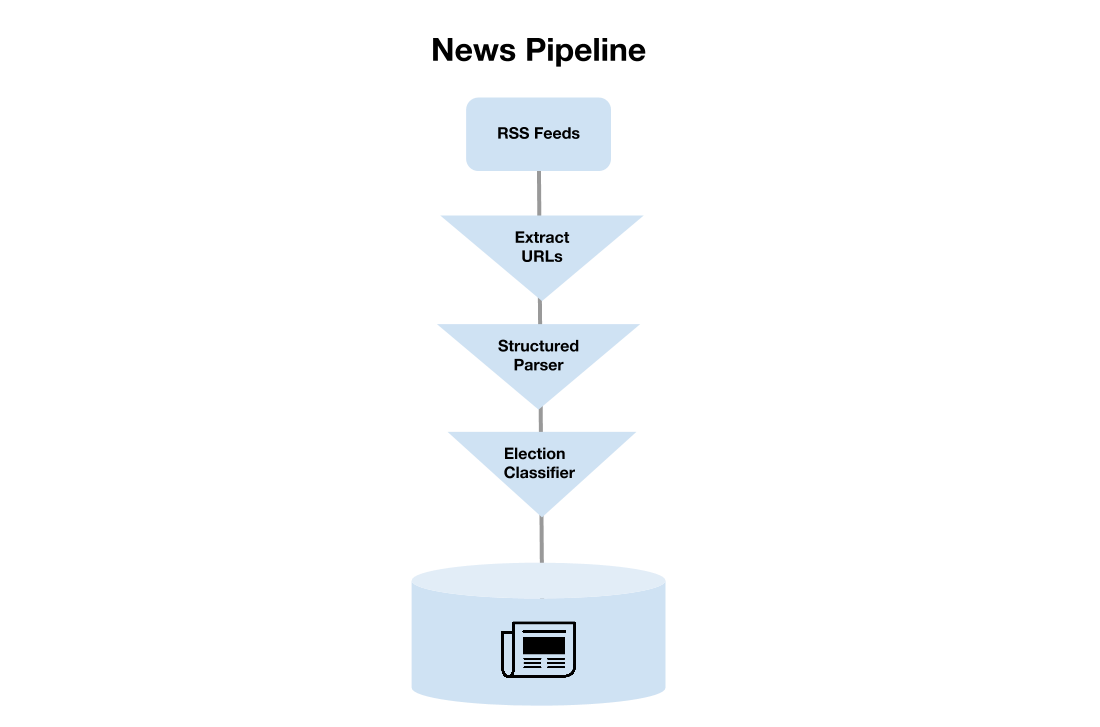
\includegraphics[width=0.9\textwidth]{election-news-pipeline}  
  \caption{Election News Pipeline
    \label{fig:data-stack}}
\end{figure}

After collecting the links to the full content of the news stories from each publication's RSS feed, we pass each link to a structured content parser that extracts entities and features from the raw HTML.

The story text is then passed into a machine learning classifier for election news from the Electome project \footnote{Designed and implemented by Prashanth Vijayaraghavan.}. 


 We collect and classify a total of 22,959 articles as election-related with over 80\% confidence, an average of 5,700 per month and 191 per day.


\section{Tweets Dataset}

\subsection{Duration \& Scope} 
The Laboratory for Social Machines was founded on the premise of a research grant with Twitter which allows access to the ``firehose'' of all activity on Twitter. We start with the pool of all tweets between January 1, 2016 and May 1, 2016 in our data process.

\subsection{Data Pipeline}

Tweets pass through a similiar pipeline as news stories. We sort all tweets with an election classifier which has been shown to be able to detect election-related tweets with an F-score of 92\% \cite{vijayaraghavan2016automatic}. We then filter by those that share a link (which might potentially be a news story).

\begin{figure}[H]  
\centering 
  \includegraphics[width=0.9\textwidth]{Twitter-pipeline}  
  \caption{Election Tweets Pipeline
    \label{fig:data-stack-Twitter}}
\end{figure} 

We collect and sort a total of 16,667,685 tweets as election-related and containing at least one URL in the text, an average of 4,000,000 per month and 140,000 per day.

\section{Combined Dataset}
The final step of our data collection process is to extract, expand and connect the links shared in our election-related tweets with articles in our database.
 
\subsection{Mapping Tweets to Stories}
\begin{figure}[H]  
\centering 
  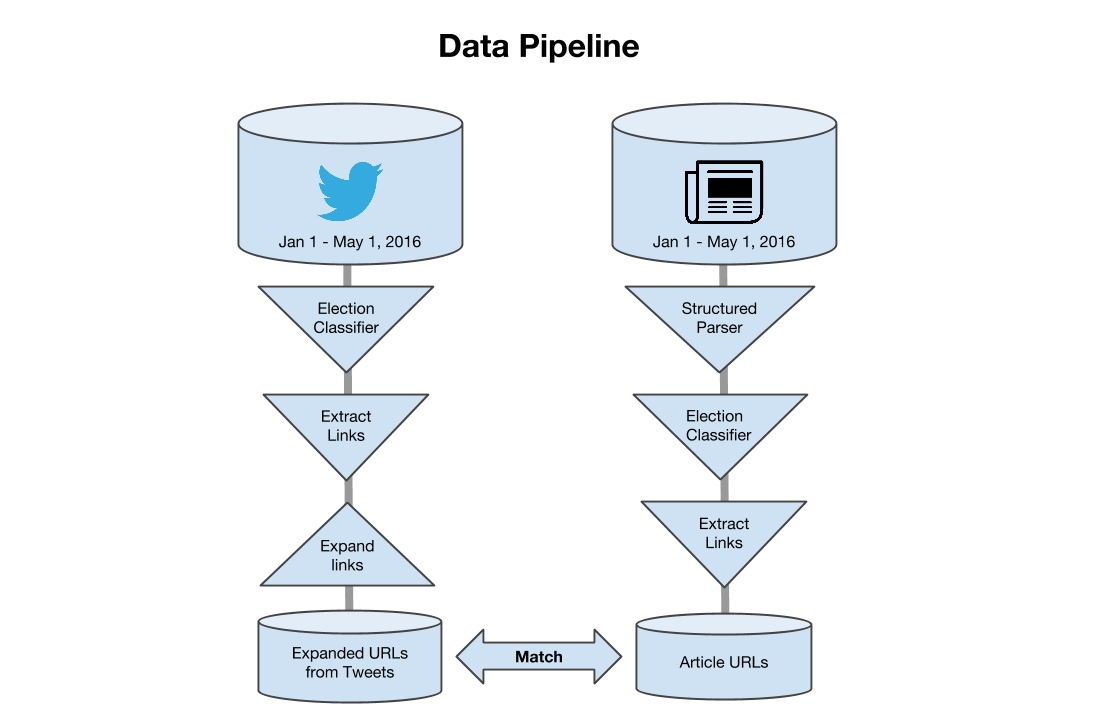
\includegraphics[width=0.9\textwidth]{data-stack}  
  \caption{Data Pipeline
    \label{fig:data-stack}}
\end{figure}
 
Twitter automatically formats all links into a shortened ``t.co'' format, so we first expand all links in tweets (16.6 million), then use a regular expression to see if the final destination of the expanded link matches a query-truncated URL of a story in our database. We checked the validity of 382 billion url-story matches in less than a day by running the processes on the Amazon Web Services cloud computing platform in parallel using the Gnu-parallel command line tool \cite{tange2011gnu}.

\subsection{Final Corpus}

In total, we found that 30\% of the election stories we tracked were shared on Twitter during the time period of January 1st through May 1st.

There were 137,986 tweets that contained a link to 6,911 unique stories (out of 22,960).

Since we chose the story to be the unit of analysis in this thesis, we then eliminated any stories that were shared by less than 10 tweets.

This left a total of 2,658 distinct articles (38\%) shared in 123,113 (89\%) tweets by 20,956 Twitter users (93\%).

 






















